\documentclass[aps,superscriptaddress]{revtex4}
\usepackage[pdftex]{graphicx}   % for figures
\usepackage{epstopdf}
\usepackage{dcolumn}
\usepackage{bm}	
\usepackage{ textcomp }
\usepackage{amsmath}			% Mode math\ufffdmatique
\usepackage{amsfonts}			% Polices math\ufffdmatiques
\usepackage{amssymb}
%\usepackage[labelformat=empty]{caption}
% Symboles math\ufffdmatiques
\usepackage{latexsym}			% Symboles math\ufffdmatiques avanc\ufffds
\usepackage{color}
% Asked by the editor
%%%%%%%%%%%%%%%%%%%%%
%\usepackage[nomarkers,figuresonly]{endfloat}
%\linespread{2}
%%%%%%%%%%%%%%%%%%%%%
%%%%%%%%%%%%%% For submission %%%%%%%%%%%
%  \renewcommand{\baselinestretch}{2} 
%%%%%%%%%%%%%%%%%%%%%%%%%%%%%%%%%%%%%%%%%
\begin{document}
\title{Supplementary information for 
``Growth of concomitant laser-driven collisionless and resistive electron filamentation instabilities over large spatiotemporal scales''
}


\author{C. Ruyer}\email{charles.ruyer@cea.fr}
\affiliation{LULI - CNRS, CEA, UPMC Univ Paris 06: Sorbonne Universit\'e, Ecole Polytechnique, Institut Polytechnique de Paris - F-91128 Palaiseau Cedex, France}
\affiliation{SLAC National Accelerator Laboratory, Sand Hill Road, Menlo Park, California, USA}
\affiliation{CEA, DAM, DIF, F-91297 Arpajon, France}
\author{S. Bolanos }
\affiliation{LULI - CNRS, CEA, UPMC Univ Paris 06: Sorbonne Universit\'e, Ecole Polytechnique, Institut Polytechnique de Paris - F-91128 Palaiseau Cedex, France}
\author{B. Albertazzi}%\email{Bruno.albertazzi@polytechnique.edu}
\affiliation{LULI - CNRS, CEA, UPMC Univ Paris 06: Sorbonne Universit\'e, Ecole Polytechnique, Institut Polytechnique de Paris - F-91128 Palaiseau Cedex, France}
\affiliation{INRS-EMT, Varennes, Qu\'ebec, Canada}
\author{S.~N. Chen}
\affiliation{ELI-NP, ”Horia Hulubei” National Institute of Physics and Nuclear Engineering, Bucharest - Magurele, Romania }
\affiliation{Institute of Applied Physics, 46 Ulyanov Street, 603950 Nizhny Novgorod, Russia}
\author{P. Antici}
\affiliation{INRS-EMT, Varennes, Qu\'ebec, Canada}
\author{J. B\"oker}
\affiliation{Institut f\"ur Laser-und Plasmaphysik, Heinrich-Heine-Universit\"at, D\"usseldorf, Germany}
\author{V. Dervieux}
\affiliation{LULI - CNRS, CEA, UPMC Univ Paris 06: Sorbonne Universit\'e, Ecole Polytechnique, Institut Polytechnique de Paris - F-91128 Palaiseau Cedex, France}
\affiliation{CEA, DAM, DIF, F-91297 Arpajon, France}
\author{ L. Lancia}
\affiliation{LULI - CNRS, CEA, UPMC Univ Paris 06: Sorbonne Universit\'e, Ecole Polytechnique, Institut Polytechnique de Paris - F-91128 Palaiseau Cedex, France}
\affiliation{Dept. SBAI, Universita di Roma ``La Sapienza'', Via A. Scarpa 14 00181 Rome, Italy}
\author{M. Nakatsutsumi}
\affiliation{LULI - CNRS, CEA, UPMC Univ Paris 06: Sorbonne Universit\'e, Ecole Polytechnique, Institut Polytechnique de Paris - F-91128 Palaiseau Cedex, France}
\address{European XFEL GmbH, Holzkoppel 4, Schenefeld D-22869, Germany}
\author{L. Romagnani}
\affiliation{LULI - CNRS, CEA, UPMC Univ Paris 06: Sorbonne Universit\'e, Ecole Polytechnique, Institut Polytechnique de Paris - F-91128 Palaiseau Cedex, France}
\author{R. Shepherd}
\affiliation{Lawrence Livermore National Laboratory, Livermore, CA 94550, USA}
\author{M. Swantusch}
\affiliation{Institut f\"ur Laser-und Plasmaphysik, Heinrich-Heine-Universit\"at, D\"usseldorf, Germany}
\author{M. Borghesi}
\affiliation{School of Mathematics and Physics, Queen's University Belfast, United Kingdom}
\author{O. Willi}
\affiliation{Institut f\"ur Laser-und Plasmaphysik, Heinrich-Heine-Universit\"at, D\"usseldorf, Germany}
\author{H. P\'epin}
\affiliation{INRS-EMT, Varennes, Qu\'ebec, Canada}
\author{M. Starodubtsev}
\affiliation{Institute of Applied Physics, 46 Ulyanov Street, 603950 Nizhny Novgorod, Russia}
\author{M. Grech}
\affiliation{LULI - CNRS, CEA, UPMC Univ Paris 06: Sorbonne Universit\'e, Ecole Polytechnique, Institut Polytechnique de Paris - F-91128 Palaiseau Cedex, France}
\author{C. Riconda}
\affiliation{LULI - CNRS, CEA, UPMC Univ Paris 06: Sorbonne Universit\'e, Ecole Polytechnique, Institut Polytechnique de Paris - F-91128 Palaiseau Cedex, France}
\author{L. Gremillet}\email{laurent.gremillet@cea.fr}
\affiliation{CEA, DAM, DIF, F-91297 Arpajon, France}
\author{J. Fuchs}\email{julien.fuchs@polytechnique.edu}
\affiliation{LULI - CNRS, CEA, UPMC Univ Paris 06: Sorbonne Universit\'e, Ecole Polytechnique, Institut Polytechnique de Paris - F-91128 Palaiseau Cedex, France}
\affiliation{Institute of Applied Physics, 46 Ulyanov Street, 603950 Nizhny Novgorod, Russia}


\begin{abstract}
\end{abstract}
\maketitle
%\renewcommand\thefigure{Supplementary Figure \arabic{figure}}  
\renewcommand{\figurename}{Supplementary Figure}

\section{Fully PIC simulation of the laser-driven thin foil dynamics}
\label{sec:PI2D}

We have conducted a large-scale, collisional, fully PIC 2D simulation of a $3\,\rm \mu m$-thick Al foil irradiated by a laser pulse of $690\,\rm fs$ FWHM duration and $3.5 \times 10^{19}\,\rm W.cm^{-2}$ peak intensity, focused to a $8\,\rm \mu m$ FWHM spot. The beam is incident from the bottom left-hand side at a $30^\circ$ angle to the target normal. The pulse maximum reaches the center of the foil target ($y=0$) at $t=0$ (see Methods for further details).


Supplementary Figures~\ref{fig:PIC_las}a-f illustrate the simulation results at $t = 0.41\,\rm ps$, i.e., $1.44\,\rm ps$ after the beginning of the simulation. One can see that small-scale ($5-10\,\rm \mu m$), quasistatic (averaged over the laser cycle) electromagnetic modulations (Supplementary Figures~\ref{fig:PIC_las}b,c) have built up in the dilute plasmas expanding from the target surfaces (see the longitudinal electron current and density in Supplementary Figures~\ref{fig:PIC_las}a,d). The strongest fluctuations have developed close to the laser spot, but those of prime relevance to our study have arisen well outside this region, preferentially in the upper part of the domain ($x\simeq 50\,\rm \mu m$ and $y\simeq 75\,\rm \mu m$). There, they reach field strengths $\sim 300-500\,\rm T$, but happen to be embedded in a larger-scale $B$-field, of $\sim 1500\,\rm T$ strength, resulting from the Biermann battery mechanism \cite{PRL_Schoeffler_2014, PRL_Haines_1997}.

The above-axis location of the remotest small-scale modulations is consistent with the early-time ($t=0-1\,\rm ps$) proton radiograph shown in Supplementary Figure~\ref{fig:rcf_supp}a. The field modulations then emerging far away from the laser spot and outside the region encompassed by the Biermann battery field (i.e., the dark circular structure at the center of the radiograph), are indeed mostly concentrated to the left of the focal spot, i.e., opposite to the laser source.
Subsequently, the field fluctuations are found to develop in all directions from the laser spot (see Figure 2 of the main paper and Supplementary Figure~\ref{fig:rcf_supp}b).

In order to support the scenario that the above fluctuations originate from the Weibel instability, we have measured the ``hot'' electrons (here defined as having kinetic energies $>100\,\rm eV$). Supplementary Figure~\ref{fig:PIC_las}f plots the spatial distribution of the electron anisotropy factor, $K_x/K_y-1$ ($K_{\alpha=x,y}$ the momentum flux along the $\alpha$ axis), showing that it changes sign between the dense and dilute parts of the target. In the far off-axis, low-density plasma regions where the fluctuations are most discernible, one finds $K_x > K_y$, thus implying that the Weibel filamentation instability can locally develop with wavenumbers along the $y$ direction. Supplementary Figure~\ref{fig:PIC_las}e further indicates that there the hot-electron temperature is of $\sim 1\,\rm MeV$.

\begin{figure*}[h]
\centerline{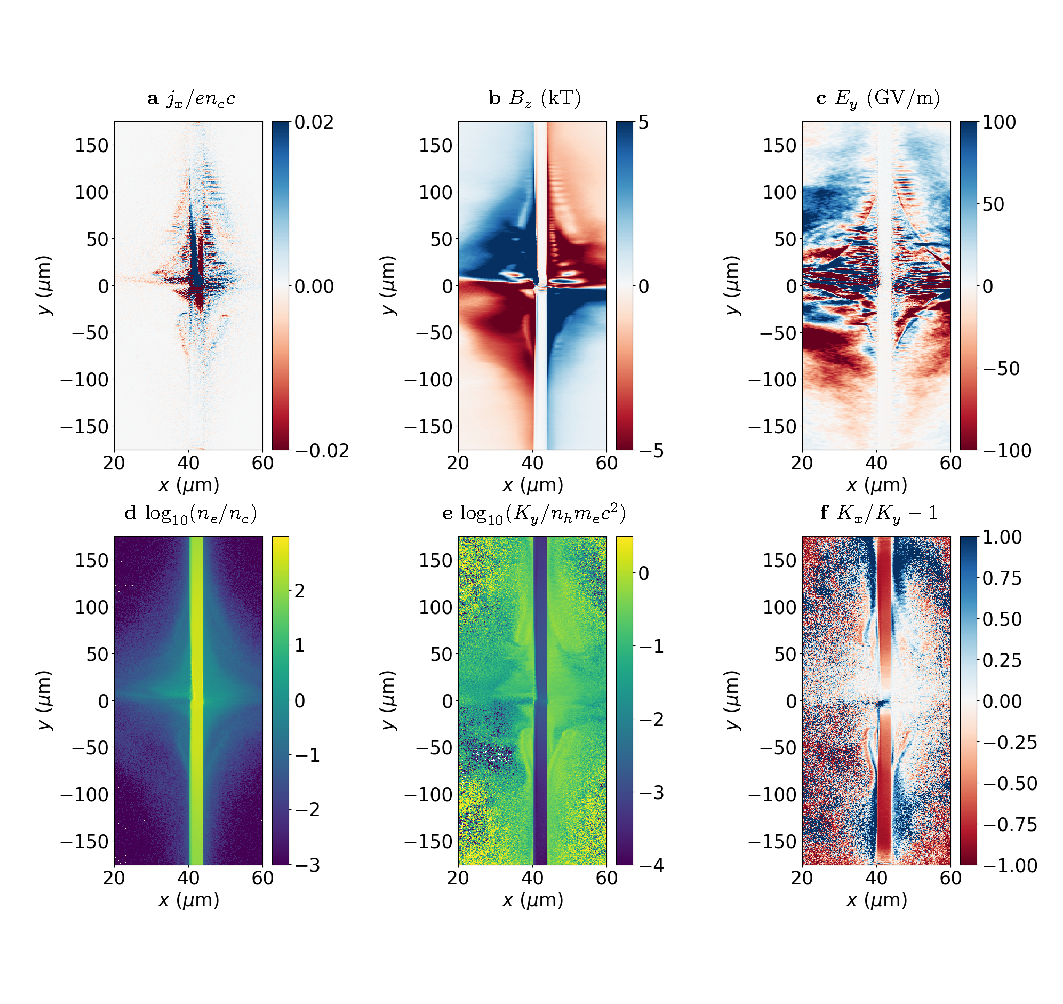
\includegraphics[width=0.95\textwidth]{FigS1.pdf} }
\caption{\label{fig:PIC_las}
{\bf Fully PIC 2D simulation of a $\boldsymbol{3\,\rm \mu m}$ Al foil driven by a $\boldsymbol{3.5 \times 10^{19}\,\rm W.cm^{-2}}$, 690~fs laser pulse.} {\bf a},~Longitudinal electron current density ($j_x$, normalized to $e n_c c$ where $n_c=1.1\times 10^{21}\,\rm cm^{-3}$ is the critical density).
{\bf b},~Out-of-plane quasistatic magnetic field ($B_z$, in kT units).
{\bf c},~Transverse quasistatic electric field ($E_y$, in $\rm GV.m^{-1}$ units).
{\bf d},~Total electron density ($n_e$, normalized to $n_c$).
{\bf e},~Transverse hot-electron temperature ($K_y$, normalized to $n_h m_ec^2$), averaged over electrons with $>100\,\rm eV$ energies.
\textbf{f},~Hot-electron anisotropy, defined as $K_x/K_y -1$, where $K_x$ (resp. $K_y$) is the hot-electron ($>100\,\rm eV$) momentum flux along $x$ (resp. $y$). All plots are recorded at $t=0.41\,\rm ps$ ($1.44\,\rm ps$ after the on-target laser pulse maximum).
}
\end{figure*}

Supplementary Figure~\ref{fig:nhcut}a presents a lineout of the hot-electron density ($n_h$) along the transverse direction ($y$) and at the longitudinal position $x=43\,\rm \mu m$. A maximum density of $n_h \sim 5 \times 10^{21}\,\rm cm^{-3}$ is reached over a $\sim 30\,\rm \mu m$ transverse extent. These values have been used to initialize the PIC-MHD simulations of the late-time hot-electron dynamics in the resistive target bulk (see Methods).

\begin{figure}[h]
\centerline{
\begin{tabular}{c}
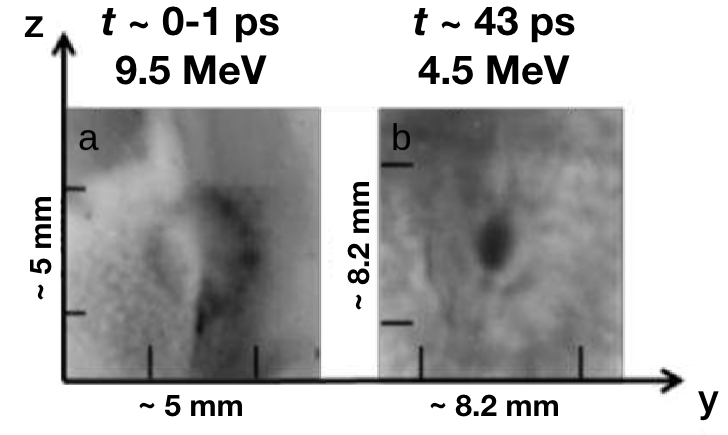
\includegraphics[scale=0.4]{FigS2.png}
\end{tabular}}
\caption{\label{fig:rcf_supp} 
\textbf{Early- and late-time experimental proton radiographs.} 
Proton radiographs of a $3\,\rm \mu m$-thick Al foil recorded at times $t\simeq 0-1\,\rm ps$ ({\bf a}) and $t\simeq 43\,\rm ps$ ({\bf b}). The laser pulse impinges from the right-hand side and is focused at the center of the radiographs, inside the dark circular structure that is induced by the surface Biermann battery $B$-field \cite{RSI_Albertazzi_2015}. The scale bars refer to the RCF plane.
}
\end{figure}

\begin{figure}[tbh!]
\centerline{
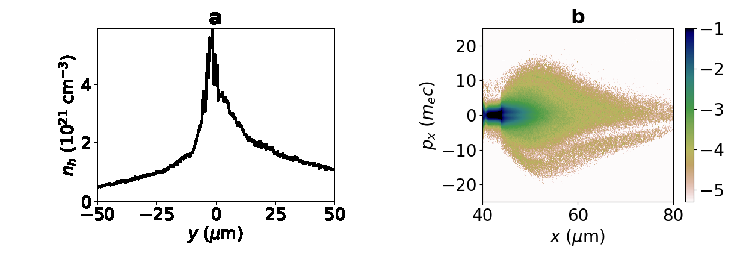
\includegraphics[width=0.8\textwidth]{FigS3.pdf} }
\caption{\label{fig:nhcut}
\textbf{Hot-electron transverse density profile and electron longitudinal phase space.}
\textbf{a}, Lineout of the hot-electron ($>100\,\rm eV$) density ($n_h$) along the transverse direction ($y$) and at $x=43\,\rm \mu m$.
\textbf{b}, Electron $x-p_x$ phase space at $y=117\,\rm \mu m$ (in $\log_{10}$ scale). Both panels are extracted at $t = 0.41\,\rm ps$ from the fully PIC 2D simulation.
}
\end{figure}

\section{Model for the collisionless filamentation instability} \label{sec:dispe_weibel}

In this section, we model the collisionless Weibel instability that generates the coupled electromagnetic and current modulations observed in Supplementary Figures~\ref{fig:PIC_las}a-c. To this purpose, following Ref.~\cite{POP_Yoon_2007b}, we describe the electrons in the expanding plasma with a two-temperature relativistic momentum distribution of the form
\begin{equation}
    f_e(\mathbf{p}) = A \exp\left[ -\frac{m_ec^2}{T_x}(\gamma -\gamma_y) -\frac{m_ec^2}{T_y}\gamma_y \right] \,,
\end{equation}
where $\gamma=\sqrt{1 + p^2/m_e^2c^2}$ and $\gamma_y=\sqrt{1 + p_y^2/m_e^2c^2}$,  
and the normalization factor $A$ is given by
\begin{equation}
    A = \frac{m_ec^2}{4\pi m_e^3c^3T_xK_2(m_ec^2T_y^{-1}) } \left[1 + \frac{T_y}{m_ec^2} \left(\frac{T_x}{T_y}-1\right)\frac{K_1(m_ec^2 T_y^{-1})}{K_2(m_ec^2T_y^{-1})} \right]^{-1} \,.
\end{equation}
In the above, $K_1(x)$ and $K_2(x)$ are modified Bessel functions of the second kind. The choice of a single (hot) electron population is motivated by the shape of the electron phase space extracted at $y=117\,\rm\mu m$ and $t=0.41\,\rm ps$ [Supplementary Figure~\ref{fig:nhcut}b], which indicates almost complete phase mixing of the high-energy electrons in the off-axis expanding plasma, except for a residual dilute stream at large negative $p_x$ values.

The linear dispersion relation of the Weibel instability with the above distribution function is given by Eq.~(5) of Ref.~\cite{POP_Yoon_2007b}. We have solved it numerically to obtain the maximum growth rate ($\Gamma_p$) and the associated wavenumber ($k_p$) (or, equivalently, wavelength $\lambda_p \equiv 2\pi/k_p$) for given values of the electron transverse temperature ($T_y$) and anisotropy factor ($T_x/T_y-1$). To facilitate extrapolation to the experimental scales, we express those quantities in terms of the hot-electron plasma frequency $\omega_{ph}$ as
\begin{align}
    \Gamma_p &= \alpha_\Gamma \omega_{ph} \label{eq:gp} \,,\\
    \lambda_p &\equiv 2\pi/k_p = 2\pi \alpha_\lambda c/\omega_{ph} \label{eq:lp}  \,,
\end{align}
where the $\alpha_\Gamma$ and $\alpha_\lambda$ proportionality factors are displayed in Supplementary Figures~\ref{fig:dispe_yoon}a,b.
From Supplementary Figures~\ref{fig:PIC_las}e,f, the electron temperature and anisotropy factor in the unstable low-density region are found to be typically $T_y/m_ec^2 \simeq 0.6$ and $T_x/T_y -1\simeq 1$ \footnote{In the PIC simulation, the temperature ratio $T_x/T_y$ at a given position is evaluated as the momentum flux ratio $K_x/K_y$, with $K_\alpha = \iiint d^3\,f_e(\mathbf{p})p_\alpha^2/\gamma$, and $f_e(\mathbf{p})$ being the local electron distribution function.}, so that $\alpha_\Gamma \simeq 0.1$ and $\alpha_\lambda \simeq 2$ (see Supplementary Figures~\ref{fig:dispe_yoon}a,b). We shall henceforth assume that the latter values also hold in the larger-scale 3D geometry of our experiment.

\begin{figure}[!t]
\centerline{
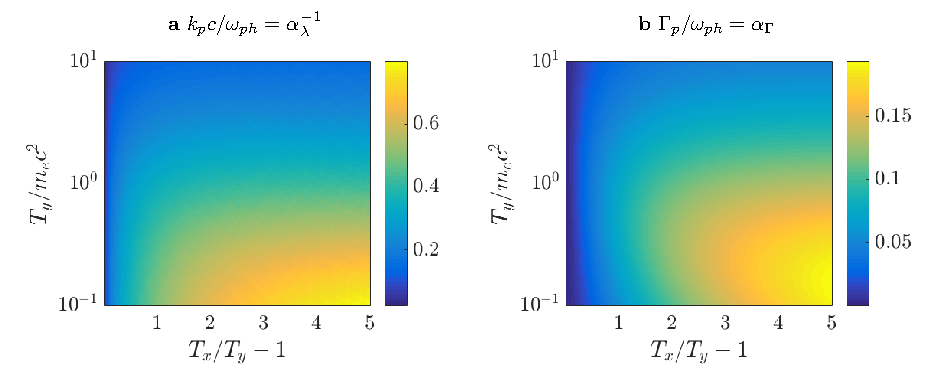
\includegraphics[width=0.9\textwidth]{FigS4.pdf}}
\caption{\label{fig:dispe_yoon}
{\bf Properties of the collisionless Weibel instability in the expanding plasma.}
{\bf a}, Most unstable wavevector.
{\bf b}, Maximum growth rate of the Weibel instability described by the dispersion relation given by Eq.~(5) of Ref.~\cite{POP_Yoon_2007b}, as a function of the hot-electron transverse temperature ($T_y/m_ec^2$) and anisotropy factor ($T_x/T_y-1$).
}
\end{figure}

\section{Model for the resistive filamentation instability} \label{sec:dispe_res}

Here, we provide a theoretical description of the filamentation instability developing in the dense resistive region of the foil target, far from the irradiated region, as a result of the counterstreaming of the hot and return-current (`cold' or `bulk') electron populations. Its dispersion relation is derived assuming the cold neutralizing electrons obey the simple Ohm's law, $\mathbf{j}_c =\sigma \mathbf{E}$, where $\mathbf{j}_c$ is the cold electron current density, $\sigma$ the electrical resistivity, and $\mathbf{E}$ the electric field. The system is taken to be infinite and uniform.

Following the standard linearization procedure of the Vlasov-Maxwell equations, the general relation fulfilled by electromagnetic fluctuations $\boldsymbol{\delta E}$ in the above two-electron-species plasma can be written as
\begin{equation}\label{eq:rose}
i \omega_{ph}^2 \int d^3 p\,\frac{\nabla_p f_h}{\omega -\mathbf{k}\cdot\mathbf{v}}\cdot \left[ \boldsymbol{\delta E} +\mathbf{v}\times\left( \frac{\mathbf{k}}{\omega} \times \boldsymbol{\delta E}\right)\right]
+ i\omega \left[ \boldsymbol{\delta E}- \frac{\sigma }{i\omega \epsilon_0}\boldsymbol{\delta E}+ \frac{\mathbf{k}c}{\omega}\times \left(\frac{\mathbf{k}c}{\omega} \times \boldsymbol{\delta E} \right) \right] =0 \,,
\end{equation}
with $\mathbf{k}$ as the (real) wavenumber, $\omega$ as the complex frequency, $f_h$ as the hot-electron momentum distribution, and $\omega_{ph}$ as the hot-electron plasma frequency.
We assume that this dispersion relation can be applied in the local $(r,\phi,x)$ Cartesian coordinates. The `longitudinal' $x$-axis is along the target normal, and $r=0$ defines the center of the hot-electron source.
The momentum distribution of the hot electrons is modeled as a multi-temperature Maxwellian,
\begin{equation}\label{eq:distrib}
f_h(v_r, v_\phi, v_x) = \left(\frac{2\pi }{m_e}\right)^{3/2} \left( T_r T_\phi T_x \right)^{1/2} \exp \left[-\frac{m_e(v_r-v_h)^2}{2T_r} -\frac{m_ev_\phi^2}{2T_\phi} -\frac{m_ev_x^2}{2T_x} \right]\,,
\end{equation}
parameterized by the radial ($T_r$), poloidal ($T_\phi$) and longitudinal ($T_x$) temperatures, and the radial drift velocity ($v_h$). The choice of a nonrelativistic distribution is justified by the subrelativistic hot-electron energies predicted by the PIC-MHD simulations far from the laser spot (see Supplementary Figures~\ref{fig:nt}b,c).

We now restrict to the case of filamentation modes characterized by poloidal wavenumbers, $k_\phi$, and longitudinal electric-field fluctuations, $\delta E_x$ (or, equivalently, radial magnetic-field fluctuations, $\delta B_r$), as illustrated by Figure~4a. The above dispersion relation then simplifies to
\begin{equation}\label{eq:dispe}
\omega^2 \epsilon_{xx} - k_\phi^2c^2 +i\omega/\tau_E = 0 \,,
\end{equation}
where $\tau_E=\epsilon_0/\sigma$ is the charge neutralization time. The kinetic dielectric tensor component, $\epsilon_{xx}$, can be written in terms of the plasma dispersion function $\mathcal{Z}$ as~\cite{POP_Ruyer_2015} 
\begin{align}
    &\epsilon_{xx} = 1 +\left(\frac{\omega_{ph}}{\omega}\right)^2 \chi_{xx}\,,\\ 
    &\chi_{xx} = -1 + \frac{T_x}{T_\phi}\left[ 1+\xi_h \mathcal{Z}(\xi_h) \right] \,,\\
    &\xi_h = \frac{\omega}{k_\phi} \sqrt{\frac{m_e}{2T_\phi}} \,.
\end{align}
In the weakly unstable regime relevant to our study, one can expand $\mathcal{Z}$ in the $\vert \xi_h \vert \ll 1$ limit~\cite{NRL_Huba_2013},
\begin{equation}
    \mathcal{Z}(\xi) = i \sqrt{\pi}(1-\xi^2) - 2\xi +4\xi^3/3 + \mathcal{O}(\xi^5) \,.
\end{equation}
The dispersion relation for the resistive filamentation instability then reduces to a second-order polynomial equation,
\begin{equation}
  \mathcal{A}\omega^2 +\mathcal{B}\omega +\mathcal{C} = 0\,,
\label{eq:dispepoloidal}
\end{equation}
where
\begin{align}
\mathcal{A}& = i\sqrt{\frac{\pi}{2}}\frac{T_x}{T_\phi} \frac{\omega_{ph}^2}{k_\phi v_{t\phi}} -\frac{i}{\tau_E}\frac{\omega_{ph}^2}{k_\phi^2 v_{t\phi}^2} a_\phi 
+i\sqrt{\frac{\pi}{2}}\frac{\omega_{ph}^4}{k_\phi^3 v_{t\phi}^3} \frac{T_x }{T_\phi} + \frac{2i}{\tau_E} \label{eq:a} \,, \\
\mathcal{B} & = -\sqrt{\frac{\pi}{2}}\frac{T_x}{T_\phi}\frac{\omega_{ph}^2}{k_\phi v_{t\phi} \tau_E}
+\omega_{ph}^2 a_\phi-\omega_{ph}^2 \frac{c^2}{v_{t\phi}^2} -k_\phi^2 c^2 -\frac{1}{\tau_E^2} + \frac{\omega_{ph}^4}{k_\phi^2 v_{t\phi}^2}a_\phi \,, \label{eq:b} \\
\mathcal{C} & =\frac{i}{\tau_E}(\omega_{ph}^2 a_\phi -k_\phi^2c^2 )\label{eq:c} \,.
\end{align}
We have also defined $a_\phi=T_x/T_\phi-1$ and $v_{t\phi}=\sqrt{T_\phi/m_e}$. The above relations do not involve $T_r$ and $v_h$ due to our focus on radial $B$-field fluctuations and the choice of the nonrelativistic, separable distribution function Eq.~\eqref{eq:distrib}. 


The unstable solution to Eq.~\eqref{eq:dispepoloidal} is readily found to be
\begin{equation}
 \omega  = -\frac{\mathcal{B}}{2\mathcal{A}}\left(1 + \sqrt{1-\frac{4\mathcal{A}\mathcal{C}}{\mathcal{B}^2}} \right)
\label{eq:dispesol}\, .
\end{equation}

\begin{figure*}[!t]
\centerline{
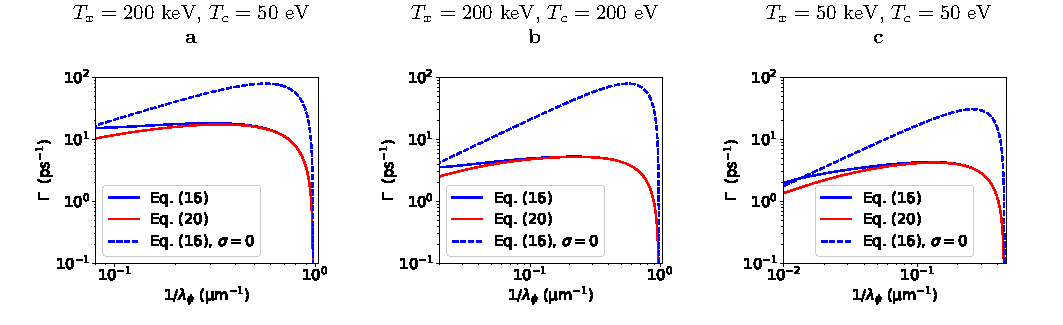
\includegraphics[width=0.99\textwidth]{FigS5.pdf} }
\caption{\label{fig:gamma_ky} 
{\bf Properties of the resistive filamentation instability in solid Al for various plasma parameters.}
{\bf a}-{\bf c}, Growth rate ($\Gamma$, in $\rm ps^{-1}$ units) vs. inverse poloidal wavelength ($\lambda_\phi^{-1}$ in $\rm \mu m^{-1}$ units). All panels consider a hot-electron density $n_h=5\times 10^{19}\,\rm cm^{-3}$ and  poloidal temperature $T_\phi=10\,\rm keV$. The other parameters are: ({\bf a}) $T_x=200\,\rm keV$ and $T_c=50\,\rm eV$, ({\bf b}) $T_x=200\,\rm keV$ and $T_c=200\,\rm eV$, ({\bf c}) $T_x=50\,\rm keV$ and $T_c=50\,\rm eV$. Solid blue curves plot Eq.~\eqref{eq:dispesol} while red curves plot the approximate formula Eq.~\eqref{eq:dispesol2}. Dashed blue curves show the limiting case of $\sigma =0$.
}
\end{figure*}

Supplementary Figures~\ref{fig:gamma_ky}a-c plot the growth rates given by Eqs.~\eqref{eq:a}-\eqref{eq:dispesol} as a function of $\lambda_\phi^{-1}$, for various plasma parameters relevant to the PIC-MHD simulations (blue solid curves). In all panels the hot-electron density and poloidal temperature are set to $n_h=5\times 10^{19}\,\rm cm^{−3}$ and $T_\phi = 10\,\rm keV$. The electrical conductivity $\sigma$ is calculated as a function of the background temperature $T_c$ following Ref.~\cite{POP_Perez_2012}. At a hot-electron longitudinal temperature $T_x=200\,\rm keV$ and a bulk electron temperature $T_c=50\,\rm eV$, corresponding to an ionization degree $Z^*\simeq 5$ \cite{More_1983} and $\sigma \simeq 10^6\,\rm S.m^{-1}$, a growth rate maximum of $\Gamma \sim 20\,\rm ps^{-1}$ is achieved at a wavelength $\lambda_\phi \simeq 2.5\,\rm \mu m$ (Supplementary Figure~\ref{fig:gamma_ky}a). Raising $T_c$ to 200~eV (Supplementary Figure~\ref{fig:gamma_ky}b) leads to $Z^* \simeq 9.3$; the associated rise in $\sigma$ (up to $\sim 5\times 10^6\,\rm S.m^{-1}$) entails a fourfold lower maximum growth rate, reached at a slightly larger $\lambda_\phi$.     

Supplementary Figures~\ref{fig:gamma_ky}a,c further show that reducing the hot-electron longitudinal temperature from $T_x=200\,\rm keV$ to 50~keV at fixed $T_\phi = 10\,\rm keV$ (i.e., decreasing the anisotropy factor by a factor of 4), and bulk temperature, $T_c=50\,\rm eV$, causes the maximum growth rate to drop from $\sim 20\,\rm ps^{-1}$ to $\sim 4\,\rm ps^{-1}$. 
For completeness, the case of a vanishing conductivity is also presented (dashed blue curves). Compared to the finite-$\sigma$ cases of $T_x=200\,\rm keV$ and $T_c=50\,\rm eV$ (Supplementary Figure~\ref{fig:gamma_ky}a) and of $T_x=200\,\rm keV$ and $T_c=50\,\rm eV$ (Supplementary Figure~\ref{fig:gamma_ky}b), the growth rate peaks at a smaller wavelength, with a maximum value larger by up to an order of magnitude -- a behavior in line with Ref.~\cite{POP_Gremillet_2002}. The instability enhancement is more moderate at $T_x=50\,\rm keV$ and $T_c=50\,\rm eV$ (\ref{fig:gamma_ky}c). The validity of the small-$\xi_h$ approximation around the $\Gamma$ maxima has been checked in all cases. 

Finally, one can derive a simple expression for the dominant resistive filamentation mode by retaining only the dominant terms of Eqs.~\eqref{eq:a}-\eqref{eq:c}. To leading order in $\omega_{ph} \tau_E \ll 1$ and $\omega_{ph}/k_\phi v_{t\phi} \ll 1$, one obtains
\begin{align}
\mathcal{A} & \simeq \frac{2i}{\tau_E}  \label{eq:a2} \,, \\
\mathcal{B} & \simeq - \sqrt{\frac{\pi}{2}}\frac{T_x }{T_\phi}\frac{\omega_{ph}^2}{k_\phi v_{t\phi} \tau_E}
 -\frac{1}{\tau_E^2} \,, \label{eq:b2} \\
\mathcal{C} & \simeq \frac{i}{\tau_E}(\omega_{ph}^2 a_\phi -k_\phi^2c^2 )\label{eq:c2} \,.
\end{align}
Substituting the above relations into Eq.~\eqref{eq:dispesol} gives
\begin{equation}
\Gamma \simeq \frac{1}{4}  \left[ \left( \sqrt{\frac{\pi}{2}} \frac{\omega_{ph}^2}{k_\phi v_{t\phi}}\frac{T_x}{T_\phi}    + \frac{1}{\tau_E} \right)^2 + 8(\omega_{ph}^2 a_\phi  - k_\phi^2 c^2 )\right]^{1/2} -\frac{1}{4} \sqrt{\frac{\pi}{2}} \frac{\omega_{ph}^2}{k_\phi v_{t\phi}}\frac{T_x}{T_\phi} - \frac{1}{4\tau_E}
\label{eq:dispesol2}\, .
\end{equation}
Supplementary Figures~\ref{fig:gamma_ky}a-c indicate that the above formula (red solid curves) correctly approximates the results obtained with the more involved expressions, Eqs.~\eqref{eq:a}-\eqref{eq:dispesol}. 

\section{Spatiotemporal evolution of the hot electrons}

\subsection{Hot-electron dynamics in low- and high-resistivity targets} 

Supplementary Figures~\ref{fig:nt}a-f present the radial profiles of the hot-electron density ($n_h$) and longitudinal/poloidal temperatures ($T_{x/\phi}$), as extracted from two PIC-MHD simulations run with $\log \Lambda=2$ (black) and $\log \Lambda=20$ (red). The other initial parameters are $R_0=32\,\rm \mu m$, $n_{h0}=5\times 10^{21}\,\rm cm^{−3}$, $T_{h0}=1\,\rm MeV$, and $T_{c0}=50\,\rm eV$ (see Methods for details). All quantities are recorded at $t=1\,\rm ps$. Overall, the two simulations yield comparable profiles outside the source region, yet the case with $\Lambda=20$ leads to higher temperatures at small radii. All curves exhibit a similar shape: a rapid drop around $r \simeq R_0$ followed by a plateau (at least up to $r\simeq 200\,\rm \mu m$).
Importantly, whereas the hot electrons are initially isotropic, they develop a substantial anisotropy in the course of their expansion: $T_\phi$ drops to a few keV outside the source region, where it is largely dominated by $T_x$, which plateaus at $\sim 100\,\rm keV$. This anisotropic configuration is vulnerable to the resistive filamentation instability, with wavenumbers along the poloidal direction, as has been addressed in Sec.~\ref{sec:dispe_res}. 

Figure~3e of the main text displays the instability growth rates ($\Gamma$) for input parameters extracted from Supplementary Figures~\ref{fig:nt}a-c: $n_h=5\times 10^{19}\,\rm cm^{-3}$, $T_x= 100\,\rm keV$, and $T_\phi=3\,\rm keV$ (resp. $T_\phi=4\,\rm keV$) for $\log \Lambda =2$ (resp. $\log \Lambda=20$). In both cases, the bulk electron temperature is fixed to $T_c=200\,\rm eV$. As expected, and in agreement with the experimental data, the largest growth rates ($\Gamma \simeq 3.5\,\rm ps^{-1}$) are obtained in the $\log \Lambda=20$ case: the dominant wavelength is $\lambda_\phi \sim 10\,\rm \mu m$, consistent with the $\sim 5-10\,\rm \mu m$ simulated values. At $\log \Lambda=2$, the $\Gamma$ curve is flatter at large $\lambda_\phi$, with a $\sim 0.7\,\rm ps^{-1}$ maximum at $\lambda_\phi\sim 10\,\rm \mu m$. We recall that the collisionless Weibel instability (see Sec.~\ref{sec:dispe_weibel}) is predicted to grow in the dilute expanding plasma ($n_h \simeq 10^{17}-10^{18}\,\rm cm^{-3}$) at a rate $\sim 0.1 \omega_{ph} \simeq 2-6\,\rm ps^{-1}$, comparable with that of the resistive filamentation instability in the bulk plasma.

\begin{figure}[!t]
\centerline{
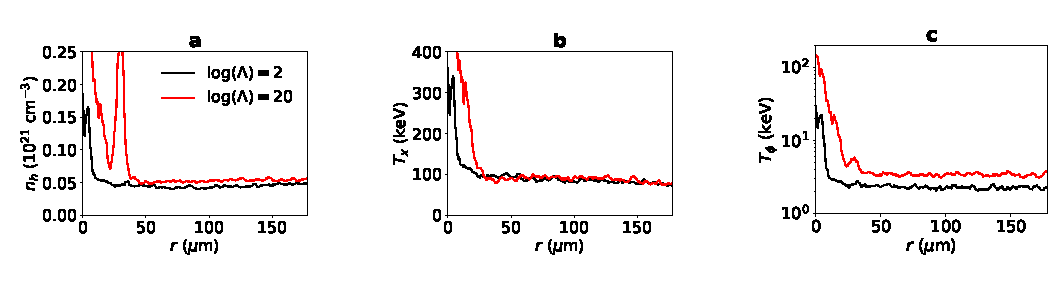
\includegraphics[width=0.98\textwidth]{FigS6.pdf} }
\caption{\label{fig:nt}
{\bf Radial profiles of the hot-electron properties from PIC-MHD simulations.}
({\bf a}), Hot-electron density ($n_h$), ({\bf b}) longitudinal temperature ($T_x$), and ({\bf c}) poloidal temperature ($T_\phi$) vs. radius.
All profiles are extracted from PIC-MHD simulations at $t=1\,\rm ps$ (see Methods). Initial parameters are $n_{h0}=5\times 10^{21}\,\rm cm ^{-3}$, $T_{h0} = 1\,\rm MeV$, $T_{c0}=50\,\rm eV$, and $R_0 = 32\,\mu\rm m$. The Coulomb logarithm is set to either $\log \Lambda=2$ (black) or $\log \Lambda=20$ (red).
}
\end{figure}

\subsection{Simple model for the hot-electron density}\label{subsec:nh}

Let us assume that the hot electrons, initially contained inside a cylinder of radius $R_0$ and length $L$ (i.e., the initial target thickness), have a density $n_{h0}$ and a temperature $T_{h0}$.
After a time $t$, they will be filling a volume of typical radius $\sim R_0 + v_{hr}t$ (in the target plane) and length $L+2c_{sh}t$ (along the target normal), where $c_{sh}=\sqrt{T_{h0}/m_\mathrm{H}}$ is the sound velocity (controlling the hot-electron-driven target expansion) and $v_{hr}$ is the effective transverse velocity ($\lesssim c$). Assuming that the hot electrons are uniformly distributed within that volume, their number density should evolve as
\begin{equation} \label{eq:nht}
n_h(r,t) \simeq \alpha_n n_{h0} \left( \frac{R_0}{R_0 + v_{hr}t } \right)^D \left( \frac{L}{L + 2c_{sh}t } \right)^\delta  H \left( 1 + \frac{v_{hr}t-r}{R_0} \right) \,.
\end{equation} 
In the above $H(r)$ denotes the step function, and $D \in (1,2)$ (resp. $\delta \in (0,1)$) are the degrees of freedom in the foil target plane (resp. along the target normal). We have also introduced $\alpha_n$ the fraction of hot electrons that effectively spread radially. $\alpha_n$ and $v_{hr}$ are treated as fitting parameters, capturing possibly significant instability and collisional effects on the electron transport.

Supplementary Figure~\ref{fig:n_param}a plots the hot-electron density profiles recorded at successive times ($t=0.65\,\rm ps$, 1.3~ps, 2.6~ps, 3.4~ps) in a MHD-PIC simulation run with $R_0=32\,\rm \mu m$, $n_{h0}=5\times 10^{21}\,\rm cm^{-3}$, $T_{h0}=1\,\rm MeV$, and $T_{c0}=50\,\rm eV$ (see Methods). Note that the longitudinal expansion is not described in this simulation (i.e., $\delta = 0$). Except for a narrow and dense central region where a large fraction of the hot electrons remain confined, the simulated profiles (solid lines) exhibit rather flat shapes at $r \gtrsim 50\,\rm \mu m$, in fair agreement with formula Eq.~\eqref{eq:nht} using $v_{hr}=0.5c$ and $\alpha_n = 0.25$ (dashed lines). The temporal evolution of the mean hot-electron density (averaged over $100<r<300\,\rm \mu m$) is plotted in Supplementary Figure~\ref{fig:n_param}b for initial bulk temperatures $T_{c0} \in (50,200)\,\rm eV$. The two $n_h$ curves show very weak dependence on $T_{c0}$.
Again, the simulation results are well reproduced by Eq.~\eqref{eq:nht}, computed with the same $\alpha_n$ and $v_{hr}$ values as above.

\begin{figure}[!t]
\centerline{
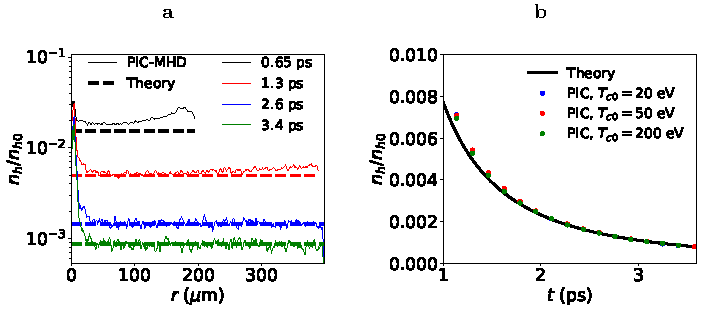
\includegraphics[width=0.66\textwidth]{FigS7.pdf} }
\caption{\label{fig:n_param} 
{\bf Spatiotemporal evolution of the hot-electron density from PIC-MHD simulations.}
{\bf a}, Radial lineouts at successive times of the hot-electron density, $n_h$, normalized to its initial value, $n_{h0}$ (solid lines), compared to the analytical estimate Eq.~\eqref{eq:nht} (dashed lines).
{\bf b}, Temporal evolution of the mean hot-electron density, $\langle n_h/n_{h0} \rangle$, averaged over $100<r<300\,\rm \mu m$. The PIC MHD simulations are initialized with $R_0=32\,\rm \mu m$, $n_{h0}=5\times 10^{21}\,\rm cm^{-3}$, $T_{h0}=1\,\rm MeV$. The bulk electron temperature is $T_{c0}=50\,\rm eV$ in {\bf a} and is varied in the $20 \le T_{c0} \le 200\,\rm eV$ range in {\bf b}. Formula~\eqref{eq:nht} is computed with $R_0=32\rm \mu m$, $v_{h0}=0.5c$, $\alpha_n=0.25$, $D=2$, and $\delta=0$. The simulation data show a negligible dependence of $\langle n_h \rangle$ on $T_{c0}$.
}
\end{figure}

\section{Proton radiographs of the Weibel filaments in the expanding plasmas} 

\subsection{Proton deflections through a Weibel-instability-induced magnetic filament}

The experimental proton radiographs show weak contrasts variations (free of caustics structures), implying that the probe protons are weakly deflected by the fields. Estimates for the deflection angle of charged particles in this regime have been derived in Ref.~\cite{RSI_protograhyb}. Of particular relevance to our problem is the case of a magnetic filament described by a ($x$-aligned) cylindrical Gaussian distribution. The filament length ($L_p$) is determined by the scale length of the expanding plasma, $L_p \simeq c_{sh}t$ (see Sec.~\ref{subsec:nh}), while the filament radius \textcolor{blue}{should scale as $a \simeq \lambda_p/4$, where $\lambda_p$ is the transverse periodicity of the $B$-field pattern.} Using Eqs.~(53), (54) and (102) of Ref.~\cite{RSI_protograhyb}, and noting that $(a^2\cos^2\theta + L_p^2 \sin^2 \theta)^{1/2} \simeq a$ ($\theta \lesssim 0.1\,\rm rad$ is the angle between the probe proton velocity and the target normal), the proton deflection angle along the transverse $z$-axis is
\begin{equation}\label{eq:alphaphith}
\theta^B_z(y_0,z_0) \simeq \pi^{1/2} y_0 \frac{L_p}{a} \frac{e B_p }{m_p v_p} \exp\left(-\frac{y_0^2+z_0^2}{a^2} \right)\,.
\end{equation}
We have introduced $m_p$ and $v_p$ the probe proton mass and velocity, and $(y_0,z_0)$ the transverse coordinates of the probe proton relative to the filament center.
The maximum value of the above expression as a function of $y_0$ and $z_0$,
\begin{equation}
\theta_{z,\rm max}^B \simeq \left(\frac{\pi}{2e_N}\right)^{1/2}\frac{e B_p L_p}{m_p v_p} \,, \label{eq:alaphaphi}
\end{equation}
depends on the filament length and magnetic field amplitude.

The Weibel instability that is held responsible for generating the magnetic filaments in the tenuous expanding plasmas is characterized by the growth rate ($\Gamma_p$) and wavelength ($\lambda_p$) given by Eqs.~\eqref{eq:gp} and \eqref{eq:lp}. A common estimate for the saturated $B$-field strength ($B_p$) is obtained by equating the instability growth rate and the electron bounce frequency inside a magnetic filament \cite{POF_Davidson_1972}:
\begin{equation}\label{eq:bp}
B_p \simeq \frac{m_e \Gamma_p^2 \lambda_p}{2\pi e v_{hx}} = \alpha_\Gamma^2 \alpha_\lambda \frac{m_e c\omega_{ph}}{e v_{hx}} \,,
\end{equation}
where $v_{hx}$ is the typical electron velocity, and $\alpha_\Gamma$ and $\alpha_\lambda$ are the proportionality factors introduced in Sec.~\ref{sec:dispe_weibel}. The Lorentz factor of the electrons driving the instability has been assumed $\sim 1$.

Evaluating Eq.~\eqref{eq:bp} with parameters relevant to the fully PIC simulation at \textcolor{blue}{$t\simeq 0.4\,\rm ps$ ($n_h \simeq 1\times 10^{20}\,\rm cm^{-3}$ and $v_{hx} = 0.5c$, see main text) yields $\lambda_p \simeq 7 \,\rm \mu m$ and $B_p \simeq 120\,\rm T$}, consistent with the wavelength and amplitude of the magnetic modulations shown in Supplementary Figure~\ref{fig:cut}a ($\lambda_p \simeq 7 \,\rm \mu m$  and \textcolor{blue}{$B_p \simeq 200-300\,\rm T$)}.

In the experiment at time $t=4\,\rm ps$, 
\textcolor{blue}{from Eq.~\eqref{eq:nht} with $(D,\delta)=(2,1)$ and $T_h\simeq 100\,\rm keV$, one expects $n_h \simeq 3\times 10^{17}\,\rm cm^{-3}$, so that $\lambda_p \simeq 110\,\rm \mu m$ and $B_p \simeq 7\,\rm T$.}
The maximum deflection angle resulting from the magnetic filaments probed along the $x$ direction is obtained by combining Eqs.~\eqref{eq:alaphaphi} and \eqref{eq:bp}:
\begin{equation} \label{eq:alaphap}
\theta_p^B \simeq \alpha_\Gamma^2 \alpha_\lambda \left(\frac{\pi}{2e_N} \right)^{1/2} \frac{m_e L_p \omega_{ph} c}{m_p v_p v_{hx}} \,. 
\end{equation}
Only considering the time dependence of the hot-electron density, and taking $L_p = c_{sh}t$, the deflection angle should vary with time as $\theta_p^B \propto (1+2c_{sh}t/L)^{-1/2}$ at $t \gg R_0/c \simeq 0.1\,\rm ps$. We therefore expect $\theta_p^B$ to slowly decrease with time as the target expands on hydrodynamical scales. This prediction is in qualitative accordance with the observed weak variations in the proton dose pattern over 10s of ps.

\begin{figure}[ht] 
\centerline{
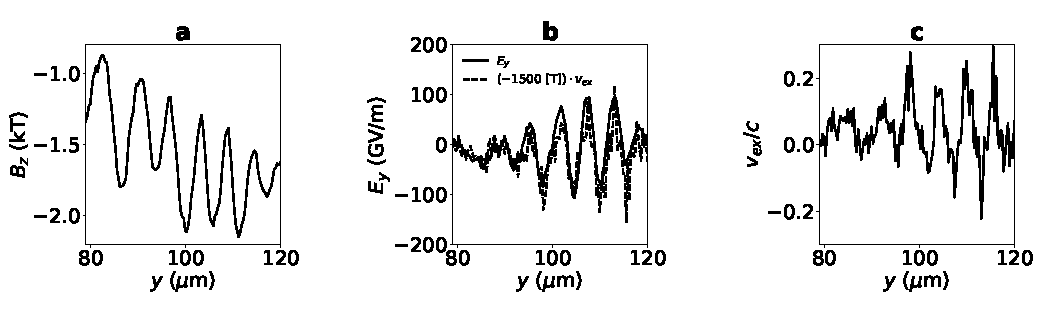
\includegraphics[width=1\textwidth]{FigS8.pdf} }
\caption{\label{fig:cut} 
\textbf{Transverse profiles of the electromagnetic fields and electron mean velocity in the expanding plasma.}
Lineouts at $x=48\,\rm \mu m$ of the ({\bf a}) $B_z$ magnetic-field component (in kT units), ({\bf b}) $E_y$ electric-field component (in $\rm GV.m^{-1}$ units), and ({\bf c}) mean electron longitudinal velocity ($v_{ex}/c$). All quantities are recorded at $t=0.41\,\rm ps$ from the 2D PIC simulation described in Sec.~\ref{sec:PI2D}. In {\bf b}, the dashed line plots the product $-1500\,[\mathrm{T}] \times v_{ex}/c$, where -1500~T is the typical strength of the large-scale Biermann battery field as estimated from {\bf a}.
}
\end{figure}

\subsection{Contribution of electric fields to proton deflections}
\label{subsec:elec_deflec}

We address here the sensitivity of the probe proton deflections to the electric fields that develop around the current filaments in the expanding plasma. Indeed, although of mainly magnetic nature, the Weibel instability can induce electric fields in its nonlinear phase (see Supplementary Figure~\ref{fig:PIC_las}c), which may affect the proton radiographs. Assuming that the unstable (hot) electron system has reached a quasi-steady state, the strength of the Weibel-generated $E$-field is estimated to be
\begin{equation} \label{eq:Ey_Weibel}
    E_y \simeq - (j_{hx} B_z + \partial_y P_h)/(en_h) \,,
\end{equation}
where $j_{hx}$ and $P_h$ are the hot-electron current density and pressure.
In our fully PIC 2D simulation (see Sec.~\ref{sec:PI2D}), the pressure term appears to be sub-dominant. The $B$-field distribution in the unstable dilute plasma comprises two components (see Supplementary Figure~\ref{fig:cut}a): short-scale Weibel fluctuations of amplitude \textcolor{blue}{$B_p \simeq 200-300\,\rm T$} and wavelength $\lambda_p \simeq 7\,\rm \mu m$, embedded inside  a large-scale field $B_b \simeq -1500\,\rm T$ due to the Biermann battery mechanism. The PIC-simulated electric field should thus scale as $E_p^{\rm PIC} \simeq v_{hx} B_b -\nabla B_p^2/(2\mu_0 e n_e) \simeq v_{hx}B_b$. This relation is confirmed to good accuracy by Supplementary Figure~\ref{fig:cut}b, which compares the transverse profiles of $E_y$ (solid curve) with $v_{hx}B_b$ (dashed curve). Therefore, over the limited scales of the 2D simulation, the $E$-field resulting from the Weibel instability is generated through the coupling of the instability-modulated electron current density and the Biermann-battery field.

That picture is expected to be altered in the experiment. There, from the radiographs of Figure~2, the Biermann battery field extends over radii $r \lesssim 200\,\rm \mu m$. Since the unstable plasma we are interested in lies well outside this region, the magnetic pressure term should now prevail over the ${\bf v}\times {\bf B}$ term in Eq.~\eqref{eq:Ey_Weibel}, so that $E_p \simeq -\nabla B_p^2/(2\mu_0 e n_e)$. \textcolor{blue}{Using our model $B$-field profile [Eq.~(5) of the main text] yields the radial $E$-field profile [Eq.~(6) of the main text] considered in \textsc{ilz} computations (see below).}

The above-discussed radial electric field tends to counteract the pinching magnetic force on the electrons, and so points toward the center of each current filament in the expanding plasma. The protons traversing a current filament are therefore \textcolor{blue}{electrically} pinched toward its center independently of the current sign (i.e., regardless of its being induced by the outgoing or ingoing electrons) or the location (front or rear target side) of the filament. This behavior contrasts with the magnetic deflections undergone by the probe protons, their focusing or defocusing effect depending on both the current sign and the target side considered. Indeed, at the rear (resp. front) side, the filaments carrying ingoing electrons tend to focus (resp. defocus) the protons, and \emph{vice versa} for those carrying outgoing electrons (see Figure~2e of the main paper).

\textcolor{blue}{We have employed the \textsc{ilz} particle-tracing code to generate synthetic radiographs under our experimental conditions (see Methods). In order to reproduce the measurements, those computations must take account of both the focusing and defocusing azimuthal $B$-field structures (resulting, respectively, in the observed black and white spots in the radiographs). The field profiles characterizing each filament are given by Eqs.~(6) and (7) of the main text. The parameters $B_0$ and $a \simeq \lambda_p/4$, though likely correlated (through the hot-electron plasma frequency), have been treated as independent when fitting the radiographic data (see Methods). The inferred parameters $(B_0,a,\lambda_p)=(5\,\rm T,30\,\rm \mu m,120\,\rm \mu m)$ yield the radiographs shown in Figures~4b,c of the main text, in fair agreement with the measurements, and it was checked that the electric field then hardly contributes to the simulated dose modulations.
}

\subsection{Influence of the magnetic field topology on the radiographs}

\begin{figure}[!t]
\centerline{
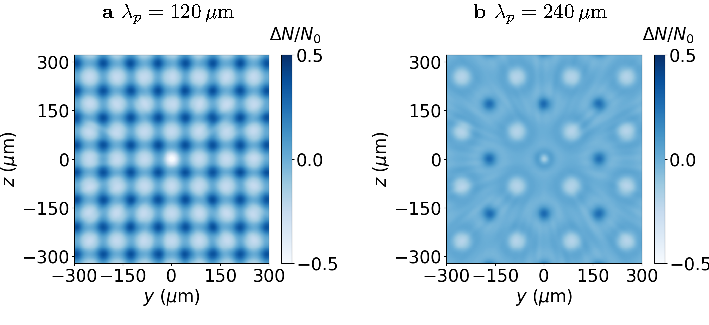
\includegraphics[width=0.66\textwidth]{FigS9.pdf} }
\caption{\label{fig:radiosup}
\textbf{Influence of the Weibel filament wavelength on the proton radiographs.}
Synthetic radiographs obtained using the \textsc{ilz} code. The $x$-aligned Weibel-induced current filaments are characterized by the (azimuthal) magnetic and (radial) electric profiles given by Eqs.~(6) and (7) in the Methods section, with $B_0=12\,\rm T$, $a=30\,\rm \mu m$, $L_p = 48\,\rm \mu m$. They are placed on one side of the target only. The minimum (diagonal) distance between filament centers of same magnetic polarity is either ({\bf a}) $\lambda_p=120\,\rm \mu m$ or ({\bf b}) $\lambda_p=240\,\rm \mu m$. The in-plane $B$-field fluctuations induced by the resistive filamentation (as given by a PIC-MHD simulation in Al, see Methods), are also included. All scales refer to  the target plane. 
}
\end{figure}

\textcolor{blue}{
Supplementary Figures~\ref{fig:radiosup}a,b illustrate the effect of varying the Weibel filament distance, $\lambda_p$ at fixed filament length $L_p=48\,\rm \mu m$, $B$-field strength $B_0=12\,\rm T$ and filament radius $a=30\,\rm\mu m$. 
The in-plane $B$-field structures due to the resistive filamentation (as provided by the PIC-MHD simulation \textcolor{blue}{in Al with $\log \Lambda =2$}, see Methods) are also included, yet they turn out to be filtered out by collisional scattering. 
For $\lambda_p=120\,\rm \mu m$ (Supplementary Figure~\ref{fig:radiosup}a), the resulting pattern is that of two shifted periodic arrays of dark and white spots. As $\lambda_p$ is increased to $240\,\rm \mu m$, light-dark rings encircle the white spots (Supplementary Figure~\ref{fig:radiosup}b). Qualitatively similar structures can be seen in the experimental radiographs shown in Figures~2a-c of the main paper at various times and positions, thus possibly as a consequence of a time-increasing filament wavelength.
}

A few hundreds of microns away from the irradiated region, expanding plasmas are likely to form at both the front and rear target sides. For thin enough targets like in our case, one may expect similar expansions, so that the Weibel-induced electromagnetic fields should develop at both sides with comparable wavelengths and strengths. In order to examine the contributions of the field modulations arising at both target sides to the radiographs, we have performed \textsc{ilz} simulations with two identical sets of electromagnetic filaments placed on each side (i.e., separated in the $x$ direction by $3\,\rm \mu m$). Both sets are characterized by $B_0=12\,\rm T$, $\lambda_p=120\,\rm \mu m$, $a=30\,\rm \mu m$, and $L_p=48\,\rm \mu m$.
Since there is, \emph{a priori}, no constraint on the relative position of the two filamentary patterns, we have considered, for the sake of illustration, two distinct configurations. 
\textcolor{blue}{
In the first (see Supplementary Figure~\ref{fig:radiosup2}b), the two patterns are shifted by $\lambda_p/2^{3/2}$ in the $z$ direction. The vertical lines then appearing on the synthetic radiograph result from the focusing filaments which become aligned when projected onto the detector. Interestingly, when the field patterns are shifted by half a wavelength in the $y+z$ direction (in the diagonal, see Supplementary Figure~\ref{fig:radiosup2}b), so that the magnetic field loops are anti-aligned from one side to the other, the relative dose variation decreases from $\Delta N/N_0 \simeq 0.4$ (Supplementary Figure~\ref{fig:radiosup}a) to  $\lesssim 0.1$ (Supplementary Figure~\ref{fig:radiosup2}b). 
As the magnetic contributions from both sides cancel out, 
the weak electric field deflections that was previously negligible (in  Figures~4c, Supplementary Figures~\ref{fig:radiosup}a,b and  \ref{fig:radiosup2}a), are now the cause of the predicted structures. 
Moreover, when increasing the probe proton incident angle (from $r = 0$ to $300\,\rm\mu m$), 
the deflections undergone by the protons at the target front and rear sides become increasingly asymmetric, leading to strongly deformed loops on the detector at $r \simeq 300\,\rm\mu m$.
}

\begin{figure}[!]
\centerline{
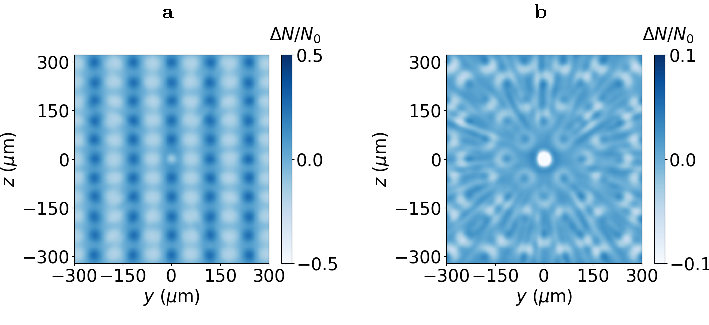
\includegraphics[width=.66\textwidth]{FigS10.pdf} }
\caption{\label{fig:radiosup2}  
\textbf{Proton radiographs of electromagnetic field patterns at both target sides.}
Synthetic radiographs obtained using the \textsc{ilz} code with the $x$-aligned Weibel filaments characterized by $B_0=12\,\rm T$, $a=30\,\rm \mu m$, $\lambda_p=120\,\rm \mu m$, and $L_p=48\,\rm \mu m$. $\lambda_p$ is the minimum (diagonal) distance between filament centers of same magnetic polarity. 
\textcolor{blue}{
Two identical electromagnetic patterns are placed at the front and rear target sides, shifted either by ({\bf a}) $\lambda_p/2^{3/2}$  along the $z$-axis or ({\bf b}) by $\lambda_p/2$  along the $y+z$ direction (diagonal). All scales refer to the target plane. 
}
}
\end{figure}


%\bibliographystyle{naturemag}
%\bibliography{biblio}

\begin{thebibliography}{10}
\expandafter\ifx\csname url\endcsname\relax
  \def\url#1{\texttt{#1}}\fi
\expandafter\ifx\csname urlprefix\endcsname\relax\def\urlprefix{URL }\fi
\providecommand{\bibinfo}[2]{#2}
\providecommand{\eprint}[2][]{\url{#2}}

\bibitem{Shkarofsky_1966}
\bibinfo{author}{Shkarofsky, I.}, \bibinfo{author}{Johnston, T.} \&
  \bibinfo{author}{Bachynski, M.}
\newblock \emph{\bibinfo{title}{The particle kinetics of plasmas}}
  (\bibinfo{publisher}{Addison-Wesley Pub. Co.}, \bibinfo{year}{1966}).

\bibitem{Belmont_2013}
\bibinfo{author}{{Belmont}, G.}, \bibinfo{author}{Roland, G.},
  \bibinfo{author}{Mottez, F.}, \bibinfo{author}{Pantellini, F.} \&
  \bibinfo{author}{Pelletier, G.}
\newblock \emph{\bibinfo{title}{{Collisionsless plasmas in astrophysics}}}
  (\bibinfo{publisher}{Wiley}, \bibinfo{year}{2013}).

\bibitem{Davidson_1983}
\bibinfo{author}{Davidson, R.~C.}
\newblock \bibinfo{title}{Kinetic waves and instabilities in uniform plasmas}.
\newblock In \bibinfo{editor}{Rosenbluth, M.~N.} \& \bibinfo{editor}{Galeev, R.~Z.} (eds.) \emph{\bibinfo{booktitle}{{Handbook of Plasma Physics}}},
  vol.~\bibinfo{volume}{1} (\bibinfo{publisher}{North-Holland},
  \bibinfo{address}{Amsterdam}, \bibinfo{year}{1983}).

\bibitem{PRL_Weibel_1959}
\bibinfo{author}{Weibel, E.~S.}
\newblock \bibinfo{title}{Spontaneous growing transverse waves in a plasma due to an anisotropic velocity distribution}.
\newblock \emph{\bibinfo{journal}{Phys. Rev. Lett.}}
  \textbf{\bibinfo{volume}{2}}, \bibinfo{pages}{83--84} (\bibinfo{year}{1959}).

\bibitem{POF_Fried_1959}
\bibinfo{author}{Fried, B.~D.}
\newblock \bibinfo{title}{Mechanism for instability of transverse plasma  waves}.
\newblock \emph{\bibinfo{journal}{Phys. Fluids}} \textbf{\bibinfo{volume}{2}},
  \bibinfo{pages}{337--337} (\bibinfo{year}{1959}).

\bibitem{POF_Davidson_1972}
\bibinfo{author}{Davidson, R.~C.}, \bibinfo{author}{Hammer, D.~A.},
  \bibinfo{author}{Haber, I.} \& \bibinfo{author}{Wagner, C.~E.}
\newblock \bibinfo{title}{Nonlinear development of electromagnetic instabilities in anisotropic plasmas}.
\newblock \emph{\bibinfo{journal}{Phys. Fluids}} \textbf{\bibinfo{volume}{15}},
  \bibinfo{pages}{317--333} (\bibinfo{year}{1972}).

\bibitem{PRL_Lee_1973}
\bibinfo{author}{{Lee}, R.} \& \bibinfo{author}{{Lampe}, M.}
\newblock \bibinfo{title}{{Electromagnetic instabilities, filamentation, and focusing of relativistic electron beams}}.
\newblock \emph{\bibinfo{journal}{Phys. Rev. Lett.}}
  \textbf{\bibinfo{volume}{31}}, \bibinfo{pages}{1390--1393}
  (\bibinfo{year}{1973}).

\bibitem{PRL_Adam_2006}
\bibinfo{author}{Adam, J.~C.}, \bibinfo{author}{H\'{e}ron, A.} \&
  \bibinfo{author}{Laval, G.}
\newblock \bibinfo{title}{Dispersion and transport of energetic particles due to the interaction of intense laser pulses with overdense plasmas}.
\newblock \emph{\bibinfo{journal}{Phys. Rev. Lett.}}
  \textbf{\bibinfo{volume}{97}}, \bibinfo{pages}{205006}
  (\bibinfo{year}{2006}).

\bibitem{RPP_Marcowith_2016}
\bibinfo{author}{{Marcowith}, A.} \emph{et~al.}
\newblock \bibinfo{title}{{The microphysics of collisionless shock waves}}.
\newblock \emph{\bibinfo{journal}{Rept. Prog. Phys.}}
  \textbf{\bibinfo{volume}{79}}, \bibinfo{pages}{046901}
  (\bibinfo{year}{2016}).

\bibitem{APJ_Schlickeiser_2003}
\bibinfo{author}{{Schlickeiser}, R.} \& \bibinfo{author}{{Shukla}, P.~K.}
\newblock \bibinfo{title}{{Cosmological magnetic field generation by the Weibel instability}}.
\newblock \emph{\bibinfo{journal}{Astrophys. J. Lett.}}
  \textbf{\bibinfo{volume}{599}}, \bibinfo{pages}{L57--L60}
  (\bibinfo{year}{2003}).

\bibitem{PRL_Allen_2012}
\bibinfo{author}{Allen, B.} \emph{et~al.}
\newblock \bibinfo{title}{Experimental study of current filamentation instability}.
\newblock \emph{\bibinfo{journal}{Phys. Rev. Lett.}}
  \textbf{\bibinfo{volume}{109}}, \bibinfo{pages}{185007}
  (\bibinfo{year}{2012}).

\bibitem{PRL_Fox_2013}
\bibinfo{author}{Fox, W.} \emph{et~al.}
\newblock \bibinfo{title}{Filamentation instability of counterstreaming laser-driven plasmas}.
\newblock \emph{\bibinfo{journal}{Phys. Rev. Lett.}}
  \textbf{\bibinfo{volume}{111}}, \bibinfo{pages}{225002}
  (\bibinfo{year}{2013}).

\bibitem{NP_Huntington_2015}
\bibinfo{author}{Huntington, C.~M.} \emph{et~al.}
\newblock \bibinfo{title}{Observation of magnetic field generation via the {Weibel} instability in interpenetrating plasma flows}.
\newblock \emph{\bibinfo{journal}{Nat. Phys.}} \textbf{\bibinfo{volume}{11}},
  \bibinfo{pages}{173--176} (\bibinfo{year}{2015}).

\bibitem{RSI_Albertazzi_2015}
\bibinfo{author}{Albertazzi, B.} \emph{et~al.}
\newblock \bibinfo{title}{A compact broadband ion beam focusing device based on laser-driven megagauss thermoelectric magnetic fields}.
\newblock \emph{\bibinfo{journal}{Rev. Sci. Instrum.}}
  \textbf{\bibinfo{volume}{86}}, \bibinfo{pages}{043502}
  (\bibinfo{year}{2015}).

\bibitem{PRL_Schoeffler_2014}
\bibinfo{author}{Schoeffler, K.~M.}, \bibinfo{author}{Loureiro, N.~F.},
  \bibinfo{author}{Fonseca, R.~A.} \& \bibinfo{author}{Silva, L.~O.}
\newblock \bibinfo{title}{Magnetic-field generation and amplification in an expanding plasma}.
\newblock \emph{\bibinfo{journal}{Phys. Rev. Lett.}}
  \textbf{\bibinfo{volume}{112}}, \bibinfo{pages}{175001}
  (\bibinfo{year}{2014}).

\bibitem{PNAS_Mondal_2012}
\bibinfo{author}{Mondal, S.} \emph{et~al.}
\newblock \bibinfo{title}{Direct observation of turbulent magnetic fields in hot, dense laser produced plasmas}.
\newblock \emph{\bibinfo{journal}{Proc. Natl. Acad. Sci. USA}} \textbf{\bibinfo{volume}{109}}, \bibinfo{pages}{8011--8015}
  (\bibinfo{year}{2012}).

\bibitem{PRL_Romagnani_2019}
\bibinfo{author}{Romagnani, L.} \emph{et~al.}
\newblock \bibinfo{title}{Dynamics of the electromagnetic fields induced by fast electron propagation in near-solid-density media}.
\newblock \emph{\bibinfo{journal}{Phys. Rev. Lett.}}
  \textbf{\bibinfo{volume}{122}}, \bibinfo{pages}{025001}
  (\bibinfo{year}{2019}).

\bibitem{POP_Gremillet_2002}
\bibinfo{author}{Gremillet, L.}, \bibinfo{author}{Bonnaud, G.} \&
  \bibinfo{author}{Amiranoff, F.}
\newblock \bibinfo{title}{Filamented transport of laser-generated relativistic electrons penetrating a solid target}.
\newblock \emph{\bibinfo{journal}{Phys. Plasmas}} \textbf{\bibinfo{volume}{9}},
  \bibinfo{pages}{941} (\bibinfo{year}{2002}).

\bibitem{JPP_Fiore_2010}
\bibinfo{author}{Fiore, M.}, \bibinfo{author}{Fiuza, F.},
  \bibinfo{author}{Marti, M.}, \bibinfo{author}{Fonseca, R.~A.} \&
  \bibinfo{author}{Silva, L.~O.}
\newblock \bibinfo{title}{Relativistic effects on the collisionless collisional  transition of the filamentation instability in fast ignition}.
\newblock \emph{\bibinfo{journal}{J. Plasma Phys.}}
  \textbf{\bibinfo{volume}{76}}, \bibinfo{pages}{813­832}
  (\bibinfo{year}{2010}).

\bibitem{POP_Yang_2016}
\bibinfo{author}{Yang, X.~H.} \emph{et~al.}
\newblock \bibinfo{title}{Effects of filamentation instability on the divergence of relativistic electrons driven by ultraintense laser pulses}.
\newblock \emph{\bibinfo{journal}{Phys. Plasmas}}
  \textbf{\bibinfo{volume}{23}}, \bibinfo{pages}{103110}
  (\bibinfo{year}{2016}).

\bibitem{PRL_Fuchs_2003}
\bibinfo{author}{Fuchs, J.} \emph{et~al.}
\newblock \bibinfo{title}{Spatial uniformity of laser-accelerated ultrahigh-current {MeV} electron propagation in metals and insulators}.
\newblock \emph{\bibinfo{journal}{Phys. Rev. Lett.}}
  \textbf{\bibinfo{volume}{91}}, \bibinfo{pages}{255002}
  (\bibinfo{year}{2003}).

\bibitem{PRL_MacLellan_2013}
\bibinfo{author}{MacLellan, D.~A.} \emph{et~al.}
\newblock \bibinfo{title}{Annular fast electron transport in silicon arising from low-temperature resistivity}.
\newblock \emph{\bibinfo{journal}{Phys. Rev. Lett.}}
  \textbf{\bibinfo{volume}{111}}, \bibinfo{pages}{095001}
  (\bibinfo{year}{2013}).

\bibitem{PRL_Storm_2009}
\bibinfo{author}{{Storm}, M.} \emph{et~al.}
\newblock \bibinfo{title}{{High-current, relativistic electron-beam transport in metals and the role of magnetic collimation}}.
\newblock \emph{\bibinfo{journal}{Phys. Rev. Lett.}}
  \textbf{\bibinfo{volume}{102}}, \bibinfo{pages}{235004}
  (\bibinfo{year}{2009}).

\bibitem{PRE_Wei_2004}
\bibinfo{author}{{Wei}, M.~S.} \emph{et~al.}
\newblock \bibinfo{title}{{Observations of the filamentation of high-intensity laser-produced electron beams}}.
\newblock \emph{\bibinfo{journal}{Phys. Rev. E}} \textbf{\bibinfo{volume}{70}},
  \bibinfo{pages}{056412} (\bibinfo{year}{2004}).

\bibitem{PRL_Quinn_2012}
\bibinfo{author}{Quinn, K.} \emph{et~al.}
\newblock \bibinfo{title}{{Weibel}-induced filamentation during an ultrafast laser-driven plasma expansion}.
\newblock \emph{\bibinfo{journal}{Phys. Rev. Lett.}}
  \textbf{\bibinfo{volume}{108}}, \bibinfo{pages}{135001}
  (\bibinfo{year}{2012}).

\bibitem{NJP_Metzkes_2014}
\bibinfo{author}{{Metzkes}, J.} \emph{et~al.}
\newblock \bibinfo{title}{{Experimental observation of transverse modulations in laser-driven proton beams}}.
\newblock \emph{\bibinfo{journal}{New J. Phys.}} \textbf{\bibinfo{volume}{16}},
  \bibinfo{pages}{023008} (\bibinfo{year}{2014}).

\bibitem{PRL_Gode_2017}
\bibinfo{author}{G\"ode, S.} \emph{et~al.}
\newblock \bibinfo{title}{Relativistic electron streaming instabilities modulate proton beams accelerated in laser-plasma interactions}.
\newblock \emph{\bibinfo{journal}{Phys. Rev. Lett.}}
  \textbf{\bibinfo{volume}{118}}, \bibinfo{pages}{194801}
  (\bibinfo{year}{2017}).

\bibitem{NJP_Scott_2017}
\bibinfo{author}{Scott, G.~G.} \emph{et~al.}
\newblock \bibinfo{title}{Diagnosis of {Weibel} instability evolution in the rear surface density scale lengths of laser solid interactions via proton  acceleration}.
\newblock \emph{\bibinfo{journal}{New J. Phys.}} \textbf{\bibinfo{volume}{19}},
  \bibinfo{pages}{043010} (\bibinfo{year}{2017}).

\bibitem{POP_Heron_2015}
\bibinfo{author}{H\'eron, A.} \& \bibinfo{author}{Adam, J.~C.}
\newblock \bibinfo{title}{Physics of the interaction of ultra intense laser pulses with cold collisional plasma using large scale kinetic simulations}.
\newblock \emph{\bibinfo{journal}{Phys. Plasmas}}
  \textbf{\bibinfo{volume}{22}}, \bibinfo{pages}{072306}
  (\bibinfo{year}{2015}).

\bibitem{NF_Lefebvre_2003}
\bibinfo{author}{Lefebvre, E.} \emph{et~al.}
\newblock \bibinfo{title}{Electron and photon production from relativistic laser-plasma interactions}.
\newblock \emph{\bibinfo{journal}{Nucl. Fusion}} \textbf{\bibinfo{volume}{43}},
  \bibinfo{pages}{629--633} (\bibinfo{year}{2003}).

\bibitem{POP_Ren_2006}
\bibinfo{author}{Ren, C.} \emph{et~al.}
\newblock \bibinfo{title}{A global simulation for laser-driven {MeV} electrons in 50-$\mu$m {Fast Ignition} targets}.
\newblock \emph{\bibinfo{journal}{Phys. Plasmas}}
  \textbf{\bibinfo{volume}{13}}, \bibinfo{pages}{056308}
  (\bibinfo{year}{2006}).

\bibitem{POP_Dieckmann_2009}
\bibinfo{author}{Dieckmann, M.~E.}, \bibinfo{author}{Kourakis, I.},
  \bibinfo{author}{Borghesi, M.} \& \bibinfo{author}{Rowlands, G.}
\newblock \bibinfo{title}{{One-dimensional particle simulation of the filamentation instability: Electrostatic field driven by the magnetic pressure gradient force}}.
\newblock \emph{\bibinfo{journal}{Phys. Plasmas}}
  \textbf{\bibinfo{volume}{16}}, \bibinfo{pages}{074502}
  (\bibinfo{year}{2009}).

\bibitem{POP_Bret_Gremillet_2010}
\bibinfo{author}{Bret, A.}, \bibinfo{author}{Gremillet, L.} \&
  \bibinfo{author}{Dieckmann, M.~E.}
\newblock \bibinfo{title}{Multidimensional electron beam-plasma instabilities in the relativistic regime}.
\newblock \emph{\bibinfo{journal}{Phys. Plasmas}}
  \textbf{\bibinfo{volume}{17}}, \bibinfo{pages}{120501}
  (\bibinfo{year}{2010}).

\bibitem{PRE_Mora_2005}
\bibinfo{author}{Mora, P.}
\newblock \bibinfo{title}{Thin-foil expansion into a vacuum}.
\newblock \emph{\bibinfo{journal}{Phys. Rev. E}} \textbf{\bibinfo{volume}{72}},
  \bibinfo{pages}{056401} (\bibinfo{year}{2005}).

\bibitem{POF_Lee_1984}
\bibinfo{author}{{Lee}, Y.~T.} \& \bibinfo{author}{{More}, R.~M.}
\newblock \bibinfo{title}{{An electron conductivity model for dense plasmas}}.
\newblock \emph{\bibinfo{journal}{Phys. Fluids}} \textbf{\bibinfo{volume}{27}},
  \bibinfo{pages}{1273--1286} (\bibinfo{year}{1984}).

\bibitem{PRL_McKenna_2011}
\bibinfo{author}{McKenna, P.} \emph{et~al.}
\newblock \bibinfo{title}{Effect of lattice structure on energetic electron transport in solids irradiated by ultraintense laser pulses}.
\newblock \emph{\bibinfo{journal}{Phys. Rev. Lett.}}
  \textbf{\bibinfo{volume}{106}}, \bibinfo{pages}{185004}
  (\bibinfo{year}{2011}).

\bibitem{PRE_Doumy_2004}
\bibinfo{author}{Doumy, G.} \emph{et~al.}
\newblock \bibinfo{title}{Complete characterization of a plasma mirror for the production of high-contrast ultraintense laser pulses}.
\newblock \emph{\bibinfo{journal}{Phys. Rev. E}} \textbf{\bibinfo{volume}{69}},
  \bibinfo{pages}{026402} (\bibinfo{year}{2004}).

\bibitem{PRL_Sarri_2012}
\bibinfo{author}{Sarri, G.} \emph{et~al.}
\newblock \bibinfo{title}{Dynamics of self-generated, large amplitude magnetic fields following high-intensity laser matter interaction}.
\newblock \emph{\bibinfo{journal}{Phys. Rev. Lett.}}
  \textbf{\bibinfo{volume}{109}}, \bibinfo{pages}{205002}
  (\bibinfo{year}{2012}).

\bibitem{RSI_Chen_2016}
\bibinfo{author}{Chen, S.~N.} \emph{et~al.}
\newblock \bibinfo{title}{Absolute dosimetric characterization of gafchromic {EBT3} and {HDv2} films using commercial flat-bed scanners and evaluation of the scanner response function variability}.
\newblock \emph{\bibinfo{journal}{Rev. Sci. Instrum.}}
  \textbf{\bibinfo{volume}{87}}, \bibinfo{pages}{073301}
  (\bibinfo{year}{2016}).

\bibitem{CPC_Sokolov_2013}
\bibinfo{author}{Sokolov, I.~V.}
\newblock \bibinfo{title}{Alternating-order interpolation in a charge-conserving scheme for particle-in-cell simulations}.
\newblock \emph{\bibinfo{journal}{Comp. Phys. Comm.}}
  \textbf{\bibinfo{volume}{184}}, \bibinfo{pages}{320 -- 328}
  (\bibinfo{year}{2013}).

\bibitem{PRSTAB_Lehe_2013}
\bibinfo{author}{Lehe, R.}, \bibinfo{author}{Lifschitz, A.},
  \bibinfo{author}{Thaury, C.}, \bibinfo{author}{Malka, V.} \&
  \bibinfo{author}{Davoine, X.}
\newblock \bibinfo{title}{Numerical growth of emittance in simulations of laser-wakefield acceleration}.
\newblock \emph{\bibinfo{journal}{Phys. Rev. ST Accel. Beams}}
  \textbf{\bibinfo{volume}{16}}, \bibinfo{pages}{021301}
  (\bibinfo{year}{2013}).

\bibitem{JCP_Vay_2011}
\bibinfo{author}{{Vay}, J.-L.}, \bibinfo{author}{{Geddes}, C.~G.~R.},
  \bibinfo{author}{{Cormier-Michel}, E.} \& \bibinfo{author}{{Grote}, D.~P.}
\newblock \bibinfo{title}{{Numerical methods for instability mitigation in the modeling of laser wakefield accelerators in a Lorentz-boosted frame}}.
\newblock \emph{\bibinfo{journal}{J. Comp. Phys.}}
  \textbf{\bibinfo{volume}{230}}, \bibinfo{pages}{5908--5929}
  (\bibinfo{year}{2011}).

\bibitem{JCP_Friedman_1990}
\bibinfo{author}{Friedman, A.}
\newblock \bibinfo{title}{{A 2nd-order implicit particle mover with adjustable damping}}.
\newblock \emph{\bibinfo{journal}{J. Comp. Phys.}}
  \textbf{\bibinfo{volume}{90}}, \bibinfo{pages}{292--312}
  (\bibinfo{year}{1990}).

\bibitem{POP_Perez_2012}
\bibinfo{author}{{P\'erez}, F.}, \bibinfo{author}{{Gremillet}, L.},
  \bibinfo{author}{Decoster, A.}, \bibinfo{author}{Drouin, M.} \&
  \bibinfo{author}{Lefebvre, E.}
\newblock \bibinfo{title}{Improved modeling of relativistic collisions and collisional ionization in particle-in-cell codes}.
\newblock \emph{\bibinfo{journal}{Phys. Plasmas}}
  \textbf{\bibinfo{volume}{19}}, \bibinfo{pages}{083104}
  (\bibinfo{year}{2012}).

\bibitem{JCP_Cohen_2010}
\bibinfo{author}{Cohen, B.}, \bibinfo{author}{Kemp, A.} \&
  \bibinfo{author}{Divol, L.}
\newblock \bibinfo{title}{Simulation of laser plasma interactions and fast-electron transport in inhomogeneous plasma}.
\newblock \emph{\bibinfo{journal}{J. Comp. Phys.}}
  \textbf{\bibinfo{volume}{229}}, \bibinfo{pages}{4591 -- 4612}
  (\bibinfo{year}{2010}).

\bibitem{PRE_Stephens_2004}
\bibinfo{author}{Stephens, R.~B.} \emph{et~al.}
\newblock \bibinfo{title}{${K}_{\ensuremath{\alpha}}$ fluorescence measurement of relativistic electron transport in the context of fast ignition}.
\newblock \emph{\bibinfo{journal}{Phys. Rev. E}} \textbf{\bibinfo{volume}{69}},
  \bibinfo{pages}{066414} (\bibinfo{year}{2004}).

\bibitem{PRL_Ping_2008}
\bibinfo{author}{Ping, Y.} \emph{et~al.}
\newblock \bibinfo{title}{Absorption of short laser pulses on solid targets in the ultrarelativistic regime}.
\newblock \emph{\bibinfo{journal}{Phys. Rev. Lett.}}
  \textbf{\bibinfo{volume}{100}}, \bibinfo{pages}{085004}
  (\bibinfo{year}{2008}).

\bibitem{Decoster_1998}
\bibinfo{author}{Decoster, A.}, \bibinfo{author}{Markowich, P.},
  \bibinfo{author}{Perthame, B.} \& \bibinfo{author}{Raviart, P.}
\newblock \emph{\bibinfo{title}{Modeling of collisions}}.
\newblock Series in applied mathematics (\bibinfo{publisher}{Gauthier-Villars},
  \bibinfo{year}{1998}).

\bibitem{NIM_Highland_1975}
\bibinfo{author}{Highland, V.~L.}
\newblock \bibinfo{title}{Some practical remarks on multiple scattering}.
\newblock \emph{\bibinfo{journal}{Nucl. Instrum. Methods}}
  \textbf{\bibinfo{volume}{129}}, \bibinfo{pages}{497 -- 499}
  (\bibinfo{year}{1975}).

\bibitem{EPJ_Groom_2000}
\bibinfo{author}{Groom, D.~E.} \& \bibinfo{author}{Klein, S.~R.}
\newblock \bibinfo{title}{Passage of particles through matter}.
\newblock \emph{\bibinfo{journal}{Eur. Phys. J. C}}
  \textbf{\bibinfo{volume}{15}}, \bibinfo{pages}{163--173}
  (\bibinfo{year}{2000}).
  
\bibitem{PRL_Haines_1997}
\bibinfo{author}{Haines, M.~G.}
\newblock \bibinfo{title}{Saturation mechanisms for the generated magnetic field in nonuniform laser-matter irradiation}.
\newblock \emph{\bibinfo{journal}{Phys. Rev. Lett.}}
  \textbf{\bibinfo{volume}{78}}, \bibinfo{pages}{254--257}
  (\bibinfo{year}{1997}).  

\bibitem{POP_Yoon_2007b}
\bibinfo{author}{Yoon, P.~H.}
\newblock \bibinfo{title}{{Relativistic Weibel instability}}.
\newblock \emph{\bibinfo{journal}{Phys. Plasmas}}
  \textbf{\bibinfo{volume}{14}}, \bibinfo{pages}{024504}
  (\bibinfo{year}{2007}).
  
\bibitem{POP_Ruyer_2015}
\bibinfo{author}{Ruyer, C.}, \bibinfo{author}{Gremillet, L.},
  \bibinfo{author}{Debayle, A.} \& \bibinfo{author}{Bonnaud, G.}
\newblock \bibinfo{title}{{Nonlinear dynamics of the ion Weibel-filamentation instability: An analytical model for the evolution of the plasma and spectral properties}}.
\newblock \emph{\bibinfo{journal}{Phys. Plasmas}}
  \textbf{\bibinfo{volume}{22}} \bibinfo{pages}{032102} (\bibinfo{year}{2015}).
  
\bibitem{NRL_Huba_2013}
\bibinfo{author}{Huba, J.~D.},
\newblock \bibinfo{title}{{NRL Plasma Formulary}},
(\bibinfo{publisher}{Naval Research Laboratory},
  \bibinfo{address}{Washington, DC}, \bibinfo{year}{2013}).
  
\bibitem{More_1983}
\bibinfo{author}{More, R.~M.}
\newblock \bibinfo{title}{Atomic Processes in High-Density Plasmas}.
\newblock In \bibinfo{editor}{Joachain, C.~J.} \& \bibinfo{editor}{Post, D.~E.} (eds.) \emph{\bibinfo{booktitle}{{Atomic Processes in High-Density Plasmas}}},
 (\bibinfo{publisher}{Springer},
  \bibinfo{address}{Boston, MA}, \bibinfo{year}{1983}).
  
\bibitem{RSI_protograhyb}
\bibinfo{author}{Kugland, N.~L.}, \bibinfo{author}{Ryutov, D.~D.},
  \bibinfo{author}{Plechaty, C.}, \bibinfo{author}{Ross, J.~S.} \&
  \bibinfo{author}{Park, H.-S.}
\newblock \bibinfo{title}{Relation between electric and magnetic field structures and their proton-beam images}.
\newblock \emph{\bibinfo{journal}{Rev. Sci. Instrum.}}
  \textbf{\bibinfo{volume}{83}}, \bibinfo{pages}{101301}
  (\bibinfo{year}{2012}).
  
\end{thebibliography}

\end{document}